%%%%%%%%%%%%%%%%%%%%%%%%%%%%%%%%%%%%%%%%%
% Journal Article
% LaTeX Template
% Version 1.4 (15/5/16)
%
% This template has been downloaded from:
% http://www.LaTeXTemplates.com
%
% Original author:
% Frits Wenneker (http://www.howtotex.com) with extensive modifications by
% Vel (vel@LaTeXTemplates.com)
%
% License:
% CC BY-NC-SA 3.0 (http://creativecommons.org/licenses/by-nc-sa/3.0/)
%
%%%%%%%%%%%%%%%%%%%%%%%%%%%%%%%%%%%%%%%%%

%----------------------------------------------------------------------------------------
%	PACKAGES AND OTHER DOCUMENT CONFIGURATIONS
%----------------------------------------------------------------------------------------

\documentclass[14pt]{article}
\usepackage[english, russian]{babel}
\usepackage{fontspec}
% \setmainfont{Times New Roman}

\setromanfont{Times New Roman}
\setsansfont{Arial}

% \usepackage{cyrtimes}

\usepackage{extsizes}
% \usepackage[T2A]{fontenc}
%
% \usepackage[utf8]{inputenc}

\usepackage{indentfirst}

%\usepackage{times}
\linespread{1.5}

\usepackage[left=3cm,right=1cm,top=1.5cm,bottom=2cm]{geometry}
\usepackage[framed,numbered,autolinebreaks,useliterate]{mcode}

\usepackage{graphicx, amsmath}
\numberwithin{figure}{section}
\graphicspath{{images/}}
\usepackage{amsfonts}
\usepackage{caption}
\captionsetup[figure]{name=Рисунок, labelsep=endash}

\numberwithin{equation}{section}

\usepackage{booktabs} % Horizontal rules in tables

\usepackage{lettrine} % The lettrine is the first enlarged letter at the beginning of the text

\usepackage{enumitem} % Customized lists
\setlist[itemize]{noitemsep} % Make itemize lists more compact

\usepackage{listings}
\lstloadlanguages{C,[ANSI]C++,Matlab}%,Clean,make,Fortran}%Загружаемые языки
\lstset{
  language=C,                % choose the language of the code
  numbers=left,                   % where to put the line-numbers
  stepnumber=1,                   % the step between two line-numbers.
  numbersep=5pt,                  % how far the line-numbers are from the code
  backgroundcolor=\color{white},  % choose the background color. You must add \usepackage{color}
  showspaces=false,               % show spaces adding particular underscores
  showstringspaces=false,         % underline spaces within strings
  showtabs=false,                 % show tabs within strings adding particular underscores
  tabsize=2,                      % sets default tabsize to 2 spaces
  captionpos=b,                   % sets the caption-position to bottom
  breaklines=false,                % sets automatic line breaking
  breakatwhitespace=false,         % sets if automatic breaks should only happen at whitespace
  frame=none,
  basicstyle=\footnotesize
  %title=\lstname,                 % show the filename of files included with \lstinputlisting;
}

\usepackage{abstract} % Allows abstract customization
\renewcommand{\abstractnamefont}{\normalfont\bfseries} % Set the "Abstract" text to bold
\renewcommand{\abstracttextfont}{\normalfont\small\itshape} % Set the abstract itself to small italic text
\newcommand{\sectionbreak}{\clearpage}
\newcommand*{\No}{\textnumero}
\renewcommand{\Re}{\mathrm{Re}}
\renewcommand{\Im}{\mathrm{Im}}

\newcommand{\const}{\mathrm{const}}
\newcommand{\arccosh}{\mathrm{arccosh}}

\newcommand{\vF}{\mathbf{F}}
\newcommand{\ve}{\mathbf{e}}
\newcommand{\vk}{\mathbf{k}}
\newcommand{\vq}{\mathbf{q}}
\newcommand{\vp}{\mathbf{p}}
\newcommand{\va}{\mathbf{a}}
\newcommand{\vP}{\mathbf{P}}
\newcommand{\vK}{\mathbf{K}}
\newcommand{\vQ}{\mathbf{Q}}
\newcommand{\vA}{\mathbf{A}}
\newcommand{\vr}{\mathbf{r}}
\newcommand{\vR}{\mathbf{R}}

\newcommand{\vRR}{\boldsymbol{\mathcal{R}}}
\newcommand{\veps}{\boldsymbol{\varepsilon}}

\newcommand{\cA}{\mathcal{A}}
\newcommand{\cR}{\mathcal{R}}
\newcommand{\cM}{\mathcal{M}}
\newcommand{\cE}{\mathcal{E}}
\newcommand{\cJ}{\mathcal{J}}
\newcommand{\cT}{\mathcal{T}}
\newcommand{\cD}{\mathcal{D}}
%\usepackage{titlesec} % Allows customization of titles
% \renewcommand\thesection{\Roman{section}} % Roman numerals for the sections
% \renewcommand\thesubsection{\roman{subsection}} % roman numerals for subsections
% \titleformat{\section}[block]{\large\scshape\centering}{\thesection.}{1em}{} % Change the look of the section titles
% \titleformat{\subsection}[block]{\large}{\thesubsection.}{1em}{} % Change the look of the section titles

% \usepackage{titling} % Customizing the title section

\usepackage{hyperref} % For hyperlinks in the PDF

\addto\captionsrussian{\def\refname{Список используемой литературы}}
\usepackage{setspace}
\onehalfspacing

\usepackage{titlesec}
\titleformat{\section}[block]{\normalsize\bfseries\centering}{\thesection}{1ex}{}
\titleformat{\subsection}[block]{\normalsize\bfseries}{\thesubsection}{1ex}{}
\titleformat{\subsubsection}[block]{\normalsize\bfseries}{\thesubsubsection}{1ex}{}

%----------------------------------------------------------------------------------------
%	TITLE SECTION
%----------------------------------------------------------------------------------------


%----------------------------------------------------------------------------------------

\begin{document}
{\sffamily

\begin{titlepage}

\thispagestyle{empty}

\newgeometry{margin=2cm}
\center

{\small МИНОБРНАУКИ РОССИИ}\\  \!  \!  \!
{\footnotesize \textbf{ФЕДЕРАЛЬНОЕ ГОСУДАРСТВЕННОЕ БЮДЖЕТНОЕ ОБРАЗОВАТЕЛЬНОЕ УЧРЕЖДЕНИЕ}}\\ \!  \!  \!
{\footnotesize  \textbf{ВЫСШЕГО ОБРАЗОВАНИЯ}}\\ \!  \!
{\small \textbf{<<ВОРОНЕЖСКИЙ ГОСУДАРСТВЕННЫЙ УНИВЕРСИТЕТ>>}}\\ \!  \!

\vspace{0.3cm}

{\small

    \centerline{Факультет \emph{компьютерных наук}}
    \vspace{0.3cm}
    \centerline{Кафедра \emph{цифровых технологий}}

    \vspace{1cm}

    \centerline{\emph{Использование метода перевала в нестационарных }}
    \centerline{\emph{задачах квантовой механики}}

    \vspace{1cm}

    \centerline{ВКР \emph{Бакалаврская работа}}
    \centerline{\emph{02.03.01 Математика и компьютерные науки}}
    \centerline{\emph{Распределенные системы и искусственный интеллект}}

    \vfill
    \begin{flushleft}
    \raggedright{Допущено к защите в ГЭК}
    \end{flushleft}
    \begin{tabbing}
    ооооооооооооооо	\=	----------------------	\kill
    Зав. кафедрой	\> 	\rule[0mm]{4cm}{0,3mm}	\emph{С.Д. Кургалин, д. ф.-м. н., профессор } \rule[0mm]{5mm}{0,3mm} . \rule[0mm]{5mm}{0,3mm} . 2017\\
    Обучающийся 	\> 	\rule[0mm]{4cm}{0,3mm}	\emph{А.А. Махно, 4 курс, д/о}             \\
    Руководитель	\> 	\rule[0mm]{4cm}{0,3mm}  \emph{А.В. Флегель, к. ф.-м. н., доцент} \\

    \end{tabbing}

    \vfill

    \centerline{Воронеж 2017}

}
\clearpage

\end{titlepage}

%----------------------------------------------------------------------------------------
%	ARTICLE CONTENTS
%----------------------------------------------------------------------------------------

%\pagestyle{plain} % нумерация вкл.
%\setcounter{page}{2} % начать нумерацию с номера два

%% ЗАДАНИЕ НА ВЫПОЛНЕНИЕ
\newpage

\thispagestyle{empty}
\newgeometry{margin=2cm}
\begin{spacing}{1.2}
{
\begin{center}

{\small МИНОБРНАУКИ РОССИИ}\\  \!  \!  \!
{\footnotesize \textbf{ФЕДЕРАЛЬНОЕ ГОСУДАРСТВЕННОЕ БЮДЖЕТНОЕ ОБРАЗОВАТЕЛЬНОЕ УЧРЕЖДЕНИЕ}}\\ \!  \!  \!
{\footnotesize  \textbf{ВЫСШЕГО ОБРАЗОВАНИЯ}}\\ \!  \!
{\small \textbf{<<ВОРОНЕЖСКИЙ ГОСУДАРСТВЕННЫЙ УНИВЕРСИТЕТ>>}}\\ \!  \!

{\small
    %\vspace{0.3cm}

    \centerline{Факультет компьютерных наук}
    \centerline{Кафедра цифровых технологий}

    \vspace{0.3cm}
}
\end{center}
{\small
    \begin{flushright} \!  \!  \! \!
    {\small УТВЕРЖДАЮ\\
    заведующий кафедрой\\
    $\underset{\text{\emph{подпись}}}{\underline{\hspace{0.15\textwidth}}}$ $\underset{\text{\emph{расшифровка подписи}}}{\underline{\text{Кургалин С.Д.,}}}$}\\
    \vspace{0.1cm}
    \rule[0mm]{5mm}{0,3mm} . \rule[0mm]{5mm}{0,3mm} . 2017\\
    \end{flushright}
    \begin{center}
    {\small \textbf{ЗАДАНИЕ \\
    НА ВЫПОЛНЕНИЕ ВЫПУСКНОЙ КВАЛИФИКАЦИОННОЙ РАБОТЫ\\
    ОБУЧАЮЩЕГОСЯ} $\underset{\text{\emph{фамилия, имя, отчество}}}{\underline{\textbf{МАХНО АРТЕМА АНДРЕЕВИЧА}}}$}
    \end{center}\! \! \!
}

\vspace{0.1cm}

{\footnotesize

    {\noindent 1. Тема работы \underline{<<Использование метода перевала в нестационарных задачах квантовой механики>>}, утверждена решением ученого совета факультета компьютерных наук от \underline{\phantom{aaa}}.\underline{\phantom{aaa}}.20\underline{\phantom{aaa}}\\
    2. { Направление подготовки / специальность $\underset{\text{\emph{шифр, наименование}}}{\underline{\text{02.03.01 Математика и компьютерные науки}}}$\\
    3. Срок сдачи студентом законченной работы \underline{\phantom{aaa}}.\underline{\phantom{aaa}}.20\underline{\phantom{aaa}}\\
    4. Календарный план: (строится в соответствии со структурой ВКР)}\\
    % \begin{tabular}[t]{|p{1em}|p{29em}|p{9em}|p{6em}|}
    \begin{tabular}[t]{|c|l|c|c|}
    \hline
        {№} & {\hspace{0.18\textwidth} Структура ВКР} & {Сроки выполнения} & {Примечание} \\
    \hline
    	{1} & {Введение}                                              & {26.10.2016} & {} \\
    \hline
    	{2} &{Глава 1. Постановка задачи}                    & {30.11.2016} & {} \\
    \hline
    	{3} &{Глава 2. Описание метода перевала \ \ \ \ \ \ \ \ \ \ \ \ \ \ \ \ \ \ \ \ \ \ \ \ \ \ \ \ \ \ \ \ \ \ \ \ \ \ \ \ }       & {16.01.2017} & {} \\
    \hline
    	{4} &{Глава 3. Решение}                              & {21.03.2017} & {} \\
    \hline
    	{5} &{Глава 4. Анализ результатов}    & {12.04.2017} & {} \\
    \hline
    	{6} &{Заключение}                                             & {3.05.2017} & {} \\
    \hline
    \end{tabular}\! \! \! \!
    \begin{flushleft}
    \vspace{0.4cm}
    {
    Обучающийся$~~~~~~~\underset{\text{\emph{подпись}}}{\underline{\hspace{0.2\textwidth}}}$ $\underset{\text{\emph{расшифровка подписи}}}{\underline{\text{Махно А.А.}\hspace{0.055\textwidth}}}$\\
    \vspace{0.4cm}
    Руководители$~~~~~~~\underset{\text{\emph{подпись}}}{\underline{\hspace{0.2\textwidth}}}$ $\underset{\text{\emph{расшифровка подписи}}}{\underline{\text{Флегель А.В.}\hspace{0.01\textwidth}}}$\\}
    \end{flushleft}\! \! \! \! \! \! \! \!

    }}
}
\end{spacing}
}


%% РЕФЕРАТ
\newpage%\thispagestyle{empty}
\addtocounter{page}{1}
\begin{center}
{\normalsize \textbf{Реферат}}
\end{center}

\begin{flushleft}
Бакалаврская работа 38 с., 17 рис.         \\
\vspace{0.5cm}

МАТЕМАТИЧЕСКОЕ МОДЕЛИРОВАНИЕ, КВАНТОВАЯ МЕХАНИКА, МЕТОД ПЕРЕВАЛА, ЧИСЛЕННОЕ ИНТЕГРИРОВАНИЕ. \\	
\vspace{0.5cm}
Объектом исследования являются интегралы от быстро осциллирующих функций, возникающие в квантово-механических задачах моделирования взаимодействия атома с лазерным импульсом. \\
\vspace{0.5cm}
Цель работы~-- получение аналитических формул для решений нестационарных уравнений квантовой механики с использованием метода перевала, а также выявление границ их применимости.\\
\vspace{0.5cm}
В процессе выполнения работы была получена аналитическая формула перевальной оценки интеграла от быстро осциллирующей функции, интенсивность осцилляций которой определяется параметрами задачи. Для получения точного результата для интеграла разработан численный метод расчета с использованием библиотек численного интегрирования. \\
\vspace{0.5cm}
В результате работы была выявлена область параметров задачи, для которой наблюдается хорошее согласие полученной аналитической оценки с исходным интегралом. Проанализированы причины нарушения согласия вне указанной области параметров. Приведенный в работе анализ может рассматриваться как одно из обоснований приближенных аналитических квазиклассических оценок в задачах квантовой механики. \\
\vspace{0.5cm}
Результаты работы могут использоваться при математическом моделировании взаимодействия атомов и молекул с интенсивными электромагнитными полями, а также в других задачах теоретической физики. 
\end{flushleft}

%\normalsize
\newgeometry{top=15mm, left=30mm, right=15mm, bottom=22mm}
\parindent = 12mm

%\newpage


\tableofcontents

\newpage

\section*{\centering Введение}
\addcontentsline{toc}{section}{Введение}

В последние годы активно развиваются высокопроизводительные вычисления с использованием массивных вычислительных кластеров и суперкомпьютеров. Область научных и технических задач, решаемых на параллельных многопроцессорных системах, стремительно расширяется и включает в себя сложные многочастичные динамические задачи, решение которых еще недавно казалось невозможным. Тем не менее, математическое и компьютерное моделирование некоторых экспериментально наблюдаемых процессов сталкивается с существенными сложностями, обусловленными, с одной стороны, все еще недостаточной мощностью вычислительных ресурсов, с другой~-- принципиальной невозможностью исключить ошибки численного решения даже при использовании наиболее продвинутых алгоритмов расчетов.  

Примером такой задачи является описание взаимодействия атомов и молекул с интенсивным низкочастотным лазерным полем, влияние которого приводит к появлению ряда нелинейных многофотонных явлений, таких как, генерация высоких гармоник лазерного поля (атом излучает фотон с энергией, в десятки или сотни раз превышающей энергию фотона поля накачки) или надпороговая ионизация атомов (электрон вырывается из связанного состояния, поглощая десятки или сотни фотонов лазерного поля). Численное решение нестационарного уравнения Шредингера, являющегося математической (квантовомеханической) моделью атома в лазерном поле, является крайне сложной задачей даже в рамках одноэлектронной модели, в которой взаимодействие активного электрона с атомным остовом описывается модельным потенциалом. Сложность этой задачи связана с экспоненциальным ростом размерности задачи (из-за роста числа узлов сетки четырехмерного пространства $\vr\otimes t$) при увеличении интенсивности лазерного поля или его длины волны. В связи с этим актуальным остается использование, во-первых, модельных подходов к описанию физики задачи, снижающих размерность исходных уравнений, и, во-вторых, приближенных методов вычислений, позволяющих получить простые аналитические результаты, удовлетворительно описывающие интересующие процессы как качественно, так и количественно. Ценность таких аналитических формул заключается также и в том, что они дают простое физическое объяснение изучаемого явления, что более трудно извлечь из ресурсозатратных вычислений.

Одним из приближенных подходов для получения аналитического результата для квантовой амплитуды многофотонного процесса в интенсивном низкочастотном лазерном поле является квазиклассический подход, основанный на использовании метода перевала. \textbf{Целью} настоящей работы является получение перевальной оценки для волновой функции атомного электрона в лазерном поле и проверка применимости такой оценки путем сравнения с точным результатом численного расчета. При формулировании проблемы, будут получены основные соотношения для волновой функции квазистационарного состояния электрона в короткодействующем потенциале и выделены временные интегралы для ключевых элементов модели. При анализе этих интегралов будут рассмотрены решения уравнений на перевальные точки подынтегральных выражений и проанализирован их вклад. Для получения точного численного результата в работе используется алгоритм на базе быстрого преобразования Фурье для интегрирования медленно затухающей осциллирующей функции.

Текст работы организован следующим образом: постановка задачи представлена в главе 1; в главе 2 описан принцип метода перевала; в главе 3 получена аналитическая формула для поставленной задачи, и анализируется метод численного интегрирования исходной функции; в главе 5 проведено сравнение численного и аналитического решения; наконец, в заключении приводятся основные результаты работы. 
\sectionbreak


\section{Постановка задачи}

В квантовой механике одноэлектронная математическая модель атома, подверженного воздействию
лазерного импульса, описывается нестационарным уравнением Шредингера для электронной волновой функции $\Psi(\vr,t)$:
\begin{equation}
\label{TDSE}
\left[i\hbar\frac{\partial}{\partial t} + \frac{\hbar^2}{2m}\nabla^2 - U(r) - V(\vr,t)\right]\Psi(\vr,t) = 0,
\end{equation}
где $U(r)$~-- потенциал взаимодействия электрона с атомным остовом, $V(\vr,t)=|e|(\vF(t)\cdot\vr)$~-- взаимодействие электрона (с зарядом $e$ и массой $m$) с лазерным импульсом, электрическое поле которого описывается вектором напряженности $\vF(t)$.\cite{7} Пусть электрон-атомное взаимодействия моделируется короткодействующим потенциалом $U(r)$, поддерживающим одно связанное сферически-симметричное состояние $\Psi_0(\vr,t)$ с энергией $E_0=-\hbar^2\kappa^2/(2m)$.

Для больших $r$, вне области действия потенциала $U(r)$ волновая функция $\Psi(\vr,t)$ ведет себя как суперпозиция расходящихся волн, соответствующих потоку уходящих на бесконечность частиц с энергиями $E=\cE(F,\omega)+n\hbar\omega$, где $\cE(F,\omega)$~-- положение атомного уровня в лазерном поле (т.е. энергия эволюционировавшего в поле $\vF(t)$ состояния $\Psi_0$), $\hbar\omega$~-- энергия лазерного фотона,  соответствующая несущей частоте $\omega$.\cite{20} Функция $\Psi(\vr,t)$ с требуемым асимптотическим поведением при $r\to\infty$ может быть выражена через нестационарную функцию Грина $G(\vr,t;\vr',t')$ для свободного электрона в поле $\vF(t)$:
\begin{equation}
\label{Psi:int}
\Psi(\vr,t) = -\frac{2\pi\hbar^2}{m\kappa}\int_{-\infty}^t
e^{-i\epsilon t'/\hbar} G(\vr,t;0,t')f(t')dt',
\end{equation}
где $f(t)$~-- неизвестная функция, которую необходимо определить из граничного условия для $\Psi(\vr,t)$ при $r\to 0$, $\epsilon$~-- квазиэнергия состояния $\Psi(\vr,t)$, переходящая в $E_0$ при выключении лазерного поля.\cite{21} Функция Грина $G(\vr,t;\vr',t')$ удовлетворяет уравнению
\begin{equation}
\label{Eq:Green}
\left[i\hbar\frac{\partial}{\partial t} + \frac{\hbar^2}{2m}\nabla^2  - V(\vr,t)\right]G(\vr,t;\vr',t') = \delta(\vr-\vr')\delta(t-t'),
\end{equation}
и имеет следующий вид:
\begin{equation}
\label{Green}
G(\vr,t;\vr',t') = -\theta(t-t')\frac{i}{\hbar}\left[\frac{m}{2\pi i\hbar(t-t')}\right]^{3/2}e^{iS(\vr,t;\vr',t')/\hbar},
\end{equation}
где $\theta(x)$~-- функция Хевисайда, и $S$~-- классическое действие для электрона в лазерном поле $\vF(t)$:
\begin{eqnarray}
S(\vr,t;\vr',t') = \frac{m}{2(t-t')}\left( \vr-\vr' -\frac{e}{mc}\int_{t'}^t\vA(\tau)d\tau \right)^2 \nonumber \\ 
-\frac{e^2}{2mc^2}\int_{t'}^t\vA^2(\tau)d\tau 
- \frac{e}{c}[\vr\vA(t)-\vr'\vA(t')].
\label{cl.S}
\end{eqnarray}
В~(\ref{cl.S}) $\vA(t)$~-- векторный потенциал лазерного поля,
\begin{equation}
\label{F-A}
\vF(t) = -\frac{1}{c}\frac{\partial\vA(t)}{\partial t}.
\end{equation}

При $r\to 0$ функция $\Psi(\vr,t)$ удовлетворяет следующему краевому условию:
\begin{equation}
\label{BC}
\Psi(\vr,t)\simeq \left(\frac{1}{r}+B(\epsilon)\right)f(t)e^{-i\epsilon t/\hbar},
\end{equation}
где явный вид зависимости $B(\epsilon)$ определяется характером взаимодействия $U(r)$. Например, для потенциала нулевого радиуса $B=-\kappa=-\sqrt{2m|E_0|}/\hbar=\mathrm{const}$.

Сшивая решение~(\ref{Psi:int}) с краевым поведением~(\ref{BC}), получим систему уравнений для коэффициентов Фурье функции $f(t)$, 
\begin{equation}
\label{forier:f}
f_n=\frac{1}{\cT}\int_0^{\cT} f(t) e^{in\omega_\tau t}dt,\quad \omega_\tau = \frac{2\pi}{\cT}, 
\end{equation}
где $\cT$~-- временной интервал между последовательными импульсами лазерного поля (рассматривается бесконечная периодическая последовательность импульсов).\cite{12}
Результирующая система уравнений для $f_n$ имеет вид:
\begin{equation}
\label{eq.system}
\sum_{n=-\infty}^\infty \cR(\epsilon+n\hbar\omega_\tau)f_ne^{-in\omega_\tau t} = \sum_{m=-\infty}^\infty e^{-im\omega_\tau t} f_m \cM(\epsilon+m\hbar\omega_\tau,t),
\end{equation}
где
\begin{equation}
\label{R}
\cR(E) = B(E) - i\sqrt{2mE}/\hbar,
\end{equation}
\begin{equation}
\label{eq:input}
\cM(\epsilon,t) = \sqrt{\frac{m}{2\pi i\hbar}}\int_0^{\infty}
\frac{e^{i\epsilon\tau/\hbar}}{\tau^{3/2}}[e^{iS(t,t-\tau)/\hbar}-1]d\tau. \cite{main}
\end{equation}

В данной работе мы анализируем ключевой элемент системы~(\ref{eq.system})~-- матричный элемент $\cM$. Используя метод перевала, будет получена аналитическая оценка для интеграла в~(\ref{eq:input}), применимость которой будет проверена численным сравнением с точным результатом для $\cM(\epsilon,t)$. В дальнейшем будет использоваться атомная система единиц, в которой $|e|=m=\hbar=1$.

Явный вид напряженности электрического поля лазерного импульса $\vF (t) = \ve_z\,F(t)$ задается следующей функцией:
\begin{equation}\label{eq:s}
S(t, t') = -\frac{1}{2}\int_{t'}^{t} [\alpha(\epsilon, t, t')]^2 d\epsilon,
\end{equation}
где
\begin{equation}\label{eq:alpha}
\alpha(\epsilon, t, t') = A(\epsilon) - \frac{1}{(t-t')}\int_{t'}^{t}A(\tau) d\tau,
\end{equation}
\begin{equation}\label{eq:a}
A(t) = -\int_{-\infty}^{t} F(\tau) d\tau.
\end{equation}
Функции $F(t)$ и $A(t)$ представлены на рисунке (\ref{ris:f_a})

\begin{figure}[h]
	\center{\includegraphics[width=0.7\linewidth]{F_A}}
	\caption{Функции $F(t)$ и $A(t)$}
	\label{ris:f_a}
\end{figure}
\sectionbreak

\section{Описание метода перевала} 

Метод перевала применяется для оценки при больших значениях параметра $\lambda$ контурных интегралов вида
\begin{equation}\label{eq:eq6}
I(\lambda) = \int_{C}^{}\phi(t)e^{\lambda f(z)}dz,
\end{equation} 
где $f(z)$ и $\phi(z)$ функции, аналитические вдоль линии интегрирования С. Интегралами вида (\ref{eq:eq6}) представляются многие специальные функции, решения дифференциальных уравнений, как обыкновенных, так и с частными производными. Эти интегралы часто встречаются при решении различных задач физики.\cite{Lavrentyev}

Рассмотрим частный случай, а именно - действительные интегралы вида

\begin{equation}\label{eq:eq7}
I(\lambda) = \int_{a}^{b}\phi(t)e^{\lambda f(t)}dt.
\end{equation} 
Этот случай был рассмотрен Лапласом. 

Предположим, что $f(t)$ имеет на отрезке $(a, b)$ один резко выраженный максимум. Чем больше значение параметра $\lambda$, тем резче выражается этот максимум, и поэтому ясно, что при больших $\lambda$ основный вклад в значение интеграла дает окрестность точки максимума. 

В основе этого метода лежит лемма:

\textit{Лемма \label{lemma:lemma1}}: Пусть дан интеграл

$$
I(\lambda) = \int_{0}^{a}\phi(t)e^{-\lambda t^\alpha}dt \:\:\:\:\:\: (0 < a \le \infty, \alpha>0),
$$
где $\phi(t)$ при $|t|<2h$ представляется сходящимся рядом

$$
\phi(t)=t^\beta(c_0+c_1 t+\dots+c_n t^n+\dots), \; \beta>-1,
$$
причем $\int_{0}^{a}|\phi(t)| e^{-\lambda_0 t^\alpha}dt\le M$ для некоторого $\lambda_0$. Тогда имеет место асимптотическое разложение

\begin{equation}\label{eq:eq8}
I(\lambda) \sim \sum_{n=0}^{\infty}\frac{c_n}{\alpha} \Gamma\left(\frac{\beta + n + 1}{\alpha}\right)\lambda^{-\frac{\beta + n + 1}{\alpha}},
\end{equation} 
где $\Gamma$ - гамма-функция Эйлера.

К доказанной лемме сводится оценка интеграла (\ref{eq:eq7}).

\textit{Теорема 1\label{th:th1}}. Пусть интеграл (\ref{eq:eq7}) абсолютно сходится для некоторого $\lambda = \lambda_0$, т. е.
$$
\int_{a}^{b} |\phi(t)|e^{\lambda_0 f(t)}dt \le M,
$$
и $f(t)$ достигает своего наибольшего значения во внутренней точке $t_0$ отрезка $(а, b)$, в окрестности $| t - t_0| < \delta$ которой $f(t)$ представляется рядом
$$
f(t)=f(t_0) + a_2(t-t_0)^2+\dots+a_n(t-t_0)^n+\dots \;\; (a_2<0),
$$
причем существует $h > 0$ такое, что вне этой окрестности $f (t_0) — f(t) > h$. Пусть еще функция $t = \psi(\tau)$ определяется в окрестности точки $\tau = 0$ из уравнения $f(t_0) — f(t) = \tau^2$, причем в этой окрестности
\begin{equation}\label{eq:eq9}
\phi[\psi(\tau)]\psi^\prime(\tau) = \sum_{n=0}^{\infty} c_n\tau^n.
\end{equation}

Тогда интеграл (\ref{eq:eq7}) имеет асимптотическое разложение
$$
I(\lambda)=\int_{a}^{b}\phi(t)e^{\lambda f(t)}dt \sim e^\lambda f(t_0) \sqrt{\frac{\pi}{\lambda}} \sum_{n=0}^{\infty}\frac{c_2n}{\lambda^n}\frac{(2n)!}{4^n n!}.
$$

Эта теорема относится к случаю, когда наибольшее значение $f(t)$ достигается во внутренней точке отрезка $(a, b)$. 

\textit{Теорема 2\label{th:th2}}. Пусть интеграл (\ref{eq:eq7}) абсолютно сходится для некоторого $\lambda = \lambda_0$ (см теорему 1) и $f(t)$ достигает наибольшего значения в точке $t=a$, аналитична в этой точке ($f^\prime(a) \neq 0$), и существует $h>0$ такое, что $f(a)-f(t)>h$ вне некоторой окрестности точки a. пусть еще функция $t=\psi(t)$ определяется в окрестности точки $\tau=0$ из уравнения $f(a) - f(t) = \tau$, причем в этой окрестности имеет место разложение (\ref{eq:eq9}). Тогда

\begin{equation}\label{eq:eq10}
I(\lambda) = \int_{a}^{b}\phi(t)e^{\lambda f(t)}dt \sim \frac{e^{f(a)}}{\lambda}\sum_{n=0}^{\infty}\frac{n! c_n}{\lambda^n}.
\end{equation}

Суть метода перевала состоит в том, что при больших значениях параметра $\lambda$ величина интеграла

$$
I(\lambda) = \int_{C}^{}\phi(t)e^{\lambda f(z)}dz
$$
в основном определяется тем участком пути интегрирования $C$, на котором $|e^{\lambda f(z)}|=e^{\lambda \Re f(z)}$, т. е. $\Re f(z)$ велика по сравнению со значениями на остальной части $С$. При этом интеграл оценивается тем легче, чем меньше этот участок и чем круче падает величина $\Re f(z)$ В соответствии со сказанным, при применении метода перевала стараются деформировать путь интегрирования С в наиболее удобный путь $\widetilde{C}$, пользуясь тем, что по теореме Коши такая деформация не меняет величины интеграла.\cite{Urmat}

Чтобы уяснить вопрос геометрически, положим $z = х + iy$, и представим
$$
u = \Re f(z),
$$
как поверхность $S$ в пространстве $(х, y, u)$. Так как функция и гармоническая, то $S$ не может иметь точек максимума и минимума, а точки, в которых $f'(z) = 0$, будут для нее точками перевала (седловыми точками, рис. \ref{ris:image2}).

\begin{figure}[h]
	\center{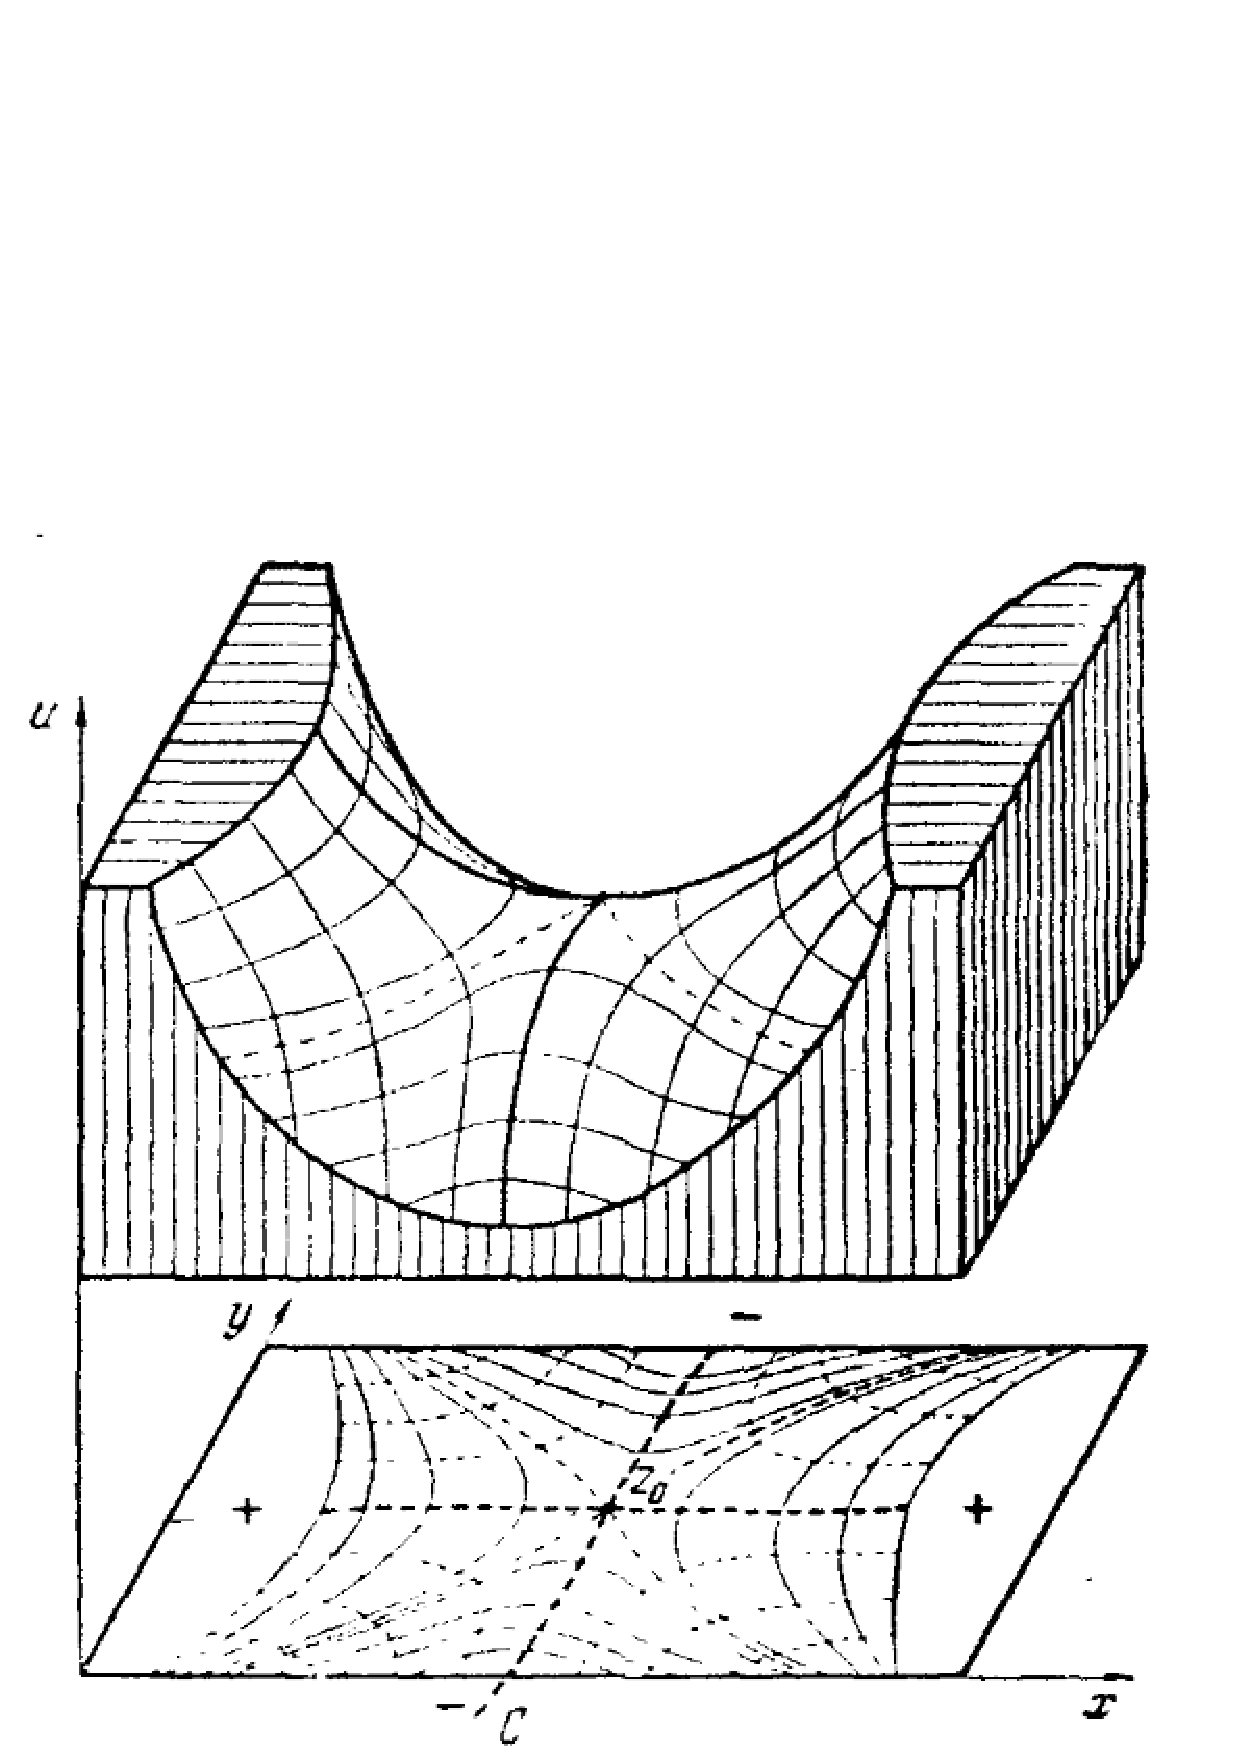
\includegraphics[width=0.3\linewidth]{pic2.png}}
	\caption{Седловые точки}
	\label{ris:image2}
	\end{figure}

Наиболее удобный для оценки путь интегрирования $\widetilde{C}$, в каждой точке должен проходить в направлении наиболее быстрого изменения $\Re f(z)$, а так как функция f(z) аналитическая, то это направление должно совпадать с линией, на которой $\Im f(z) = \const$. 

Также, новый контур $\widetilde{C}$ должен содержать точку $z_0$, в которой $\Re f(z)$ достигает наибольшего значения на $\widetilde{C}$. Покажем для этого случая, что $f^\prime (z_0) = 0$, то есть точка линии $\Im f(z) = \const$, в которой $\Re f (z)$ достигает наибольшего значения, является точкой перевала.

Так и есть, ведь в точке $z_0$, которая является максимумом для $\Re f (z)$ производная $u=0$ вдоль линии $\widetilde{C}$ должна быть равна 0, т. е. $\frac{\partial}{\partial s}\Re f(z)=0$, а так как $\Im f(z) = \const$ на $\widetilde{C}$, то $\frac{\partial}{\partial s} \Im f(z) \equiv = 0$, а значит и 

$$
f^\prime(z_0) = \frac{\partial}{\partial s} \Re f(z) + i\frac{\partial}{\partial s} \Im f(z) = 0.
$$ 

\textit{Для метода перевала к интегралу (\ref{eq:eq6}) путь интегрирования $С$ следует деформировать в путь $\widetilde{C}$, проходящий через точку перевала $z_0$ и в окрестности этой точки идущий вдоль линии наибольшего ската $\Im f(z) = \const$ (рис. \ref{ris:image2}).}

Есть одно важное обстоятельство, обеспечивающее эффективность применения метода перевала: так как вдоль линии $\widetilde{C}$ имеем $\arg e^{f(z)} = \Im f(z) = \const$, то оценка интеграла (\ref{eq:eq6}) сводится к оценке интеграла от действительной функции, которая может быть проведена по методу Лапласа для интеграла вида (\ref{eq:eq7}).  \cite{Fedoryuk}

Именно это позволяет нам пользоваться полученными результатами теорем 1 и 2. 

Рассмотрим  случай, когда путь интегрирования $С$ можно деформировать в путь $\widetilde{C}$, проходящий через точку перевала $z_0$, где $f^\prime(z_0) = 0$, $f^{\prime\prime}(z_0)\neq0$, и в окрестности $z_0$ совпадающий с линией наибольшего ската $\Im f(z) = \const$, причем на $\widetilde{C}$ вне этой окрестности $\Re f(z) < \Re f(z_0) - h \;(h> 0)$. Кроме того, предположим, что интеграл (\ref{eq:eq6}) абсолютно сходится для достаточно больших значений $\lambda$.
Тогда образом, оценку интеграла можно провести на основании теоремы 1. Пусть $z = z(t)$ будет уравнение контура $\widetilde{C}$; Тогда,

\begin{equation}\label{eq:eq11}
I(\lambda) = \int_{C}^{}\phi(z) e^{\lambda f(z)}dz=e^{\lambda i \Im f[z(t)]}\int_{a}^{b}\phi[z(t)]e^{\lambda \Re f[z(t)]}z^{\prime} dt.
\end{equation}

и задача сводится к оценки интеграла вида $\ref{eq:eq7}$ действительной области, разложение для которого уже было получено Лапласом, и имеет вид \cite{Wong}:

$$
I(\lambda) = \int_{a}^{b}\phi(t)e^{\lambda f(t)}dt \sim \frac{e^{f(a)}}{\lambda}\sum_{n=0}^{\infty}\frac{n! c_n}{\lambda^n}.
$$

Выпишем первый член этого разложения. Обозначим $\phi[z(t)]z^\prime = \widetilde{\phi}(t)$, $\Re f[z(t)] = \widetilde{f}(t)$ и тогда по формуле (\ref{eq:eq10}) получаем:

\begin{equation}\label{eq:eq12}
\int_{a}^{b} \widetilde{\phi}(t) e^{\lambda \widetilde{f}(t)}dt \sim e^{\lambda \widetilde{f}(t_0)} \sqrt{\frac{\pi}{\lambda}} \widetilde{c_0},
\end{equation}
где $\widetilde{c_0}$ - свободный член в разложении функции $\widetilde{\phi}[\widetilde{\psi}(\tau)]\widetilde{\psi^\prime}(\tau)$.

Имеем: $\widetilde{\phi}(t_0) = \phi(z_0) z^\prime (t_0)$, и исходя из того, что $f[z(t)] = \Re f[z(t)]+ i \Im f[z(t)] = \widetilde{f}(t)+\const$ вдоль $\widetilde{C}$, то

\begin{equation}\nonumber
\widetilde{f}^{\prime\prime} (t_0) = \frac{d^2}{d t^2} f[z(t)]\;|_{t=t_0} = f^{\prime\prime} (z_0) z^{\prime^2} (t_0),
\end{equation}
причем $f^\prime[z(t)] z^{\prime \prime} (t) = 0$ при $t=t_0$. Так как эта величина отрицательна, то представив $z^\prime (t_0) = k e^{i \theta}$, можно записать ее в виде $\widetilde{f}^{\prime\prime}=-|f^{\prime\prime}(z_0)| k^2$. Получаем, что 

\begin{equation}\nonumber
\widetilde{c}_0=\widetilde{\phi}(t_0) \sqrt{-\frac{2}{\widetilde{f}^{\prime\prime}(z_0)}}= \phi (z_0) e^{i \theta} \sqrt{\frac{2}{|f^{\prime\prime}(z_0)|}}.
\end{equation}
Подставим найденное значение в (\ref{eq:eq12}), а затем в (\ref{eq:eq11}), получаем искомую формулу

\begin{equation}\label{eq:eq13}
I(\lambda) \sim e^{\lambda f (z_0)}\sqrt{\frac{2\pi}{|f^{\prime \prime} (z_0)|}} \phi(z_0) e^{i \theta} \frac{1}{\sqrt{\lambda}}.
\end{equation}

Как говорилось ранее, точка $z_0$ - это точка, где $\Re f(z)$ достигает своего максимального значения. В то же время совершенно обычная ситуация - когда на искомом контуре $\widetilde{C}$ имеется несколько точек перевала, в которых значения $\Re f (z)$ находятся вблизи к наибольшему, то следует взять сумму выражений (\ref{eq:eq13}) по всем этим точками. 

Тот случай, когда контур интегрирования заканчивается в точке перевала $z_0$, аналогичным образом приводится к теореме \ref{th:th2}.

Итак, мы получили рабочую формулу, подставляя в которую составляющие наших искомых функций $\phi (z)$ и $f (z)$, мы должны получать приближенные значения интеграла, когда $\lambda \rightarrow \infty$ 

В интеграле $\cM(\epsilon,t)$ (\ref{eq:input}) роль большого параметра $\lambda$ играет конструкция вида:

\begin{equation}\label{eq.lambda}
\lambda = \frac{1}{2 \cT} \int_{-\cT/2}^{\cT/2} A^2(\tau) d\tau.
\end{equation}

\sectionbreak
\section{Методы вычисления функции $\cM(\epsilon,t)$}
\subsection{Аналитическое решение}
Получим формулу оценки интеграла (\ref{eq:input}) при помощи метода перевала.

Множитель интеграла $\frac{1}{(t-t')^{3/2}}$ приводит к тому, что в случае, когда $t \rightarrow t'$ возникает бесконечность, которую  необходимо учитывать. Конечно, в нашем случае, участок, на котором эта бесконечность возникает интересовать не должен, так как метод перевала применим для случая $\lambda \gg 1$, где $\lambda$ из формулы (\ref{eq.lambda}).  

Функция $S(t', t)$ при фиксированном t имеет вид:

Построим эту функцию 

\begin{figure}[h]
	\center{\includegraphics[width=0.7\linewidth]{S}}
	\caption{Значение функции $S(t', t)$ для t=-20, 0 и 20}
	\label{ris:S}
\end{figure}

Из рисунка (\ref{ris:S}) видно, что большое значение функция $S$ может принимать только в случае $|t - t'|\gg 1 $. Несмотря на это следует рассмотреть случай $t = t'$ отдельно, в связи с тем, что вклад этой точки может оказывать большое влияние на результат. В этом случае ($t \rightarrow t'$) разложение функции $S$ в ряд Тейлора принимает вид

$$ 
S(\tau, t) \sim \frac{1}{24} \left( \frac{d}{dt}A(t)\right)^{2}(t' - t)^3 + \frac{1}{24} \frac{d}{dt}A(t) \cdot \frac{d^2}{dt^2}A(t) (t' - t)^4 + ...
$$

При втором приближении получаем

\begin{equation}\label{eq:S_0}
S(t', t) \sim \frac{1}{24} \left( \dot{A}(t)\right)^{2}(t' - t)^3.
\end{equation}

Подставляя это $S$ в интеграл $\cM$ и введем замену $t - t' = \tau$, получаем 

\begin{eqnarray}
\cM_{\tau = 0} = \frac{1}{\sqrt{2\pi i}} \int_{0}^{\infty} \frac{e^{i \epsilon \tau}}{\tau^{3/2}} \left(e^{-i \frac{\dot{A(t)}^2}{24} \tau^3} - 1\right) d\tau  = \nonumber \\
= \frac{1}{\sqrt{2\pi i}} \int_{0}^{\infty} e^{i \epsilon \tau} \tau^{3/2} d\tau \cdot \left(-i\frac{\dot{A}(t)^2}{24}\right) \nonumber
\end{eqnarray}

Таким образом, вклад этой точки $\cM_{\tau = 0}$, при включении его в сумму учитывает элемент подынтегральной (-1), а значит при расчете остальных перевальных точек его можно не учитывать.

На рисунке \ref{ris:I_0} отображен график $\cM_{\tau = 0}$. 

\begin{figure}[h]
	\center{\includegraphics[width=0.7\linewidth]{I_0}}
	\caption{Вклад интеграла $\cM_{\tau = 0}(\epsilon, t)$}
	\label{ris:I_0}
\end{figure}

Полученная функция, как видно из графика, очень быстро затухает. Поскольку при недостаточном отдалении от нуля ($t \approx 0$) даже для функции $S(t', t)$ малый размер функции не позволяет использовать перевальную оценку, то вкладом $\cM_{\tau = 0}(\epsilon, t)$ вблизи нуля, а также на остальном участке можно пренебречь (т. к. на интервале $t = (10, \infty)$ $\cM_{\tau = 0}(\epsilon, t) = 0$).  

Тогда интеграл принимает вид:

$$
\cM \sim \int_{-\infty}^{t} \frac{1}{(t-t')^{3/2}} e^{i[\epsilon (t - t') + S(t, t')]} dt'.
$$

После замены $t - t' = \tau$, получаем 

$$
\cM \sim \int_{0}^{\infty}\frac{1}{{\tau}^{3/2}}e^{i [\epsilon \tau + S(t, t-\tau)]} d\tau.
$$

Если обозначить
$
f(t, \tau) = \epsilon \tau + S(t, t-\tau) 
$ и
$
\phi(\tau) = \frac{1}{{\tau}^{3/2}} 
$, то получим формулу вида:

$$
M \sim \int_{0}^{\infty} \phi(\tau) e^{i f(t, \tau)} d\tau.
$$

Которая совпадает с формулой для Метода Перевала, применимого для интегралов вида (\ref{eq:eq6}).

Для нашего случая приближение должно иметь вид:

$$
M_0(\epsilon, t) \simeq \sqrt{\frac{1}{2\pi i }}\sum_{t0}e^{f(t, t_0)} \sqrt{-\frac{2}{\frac{\partial f(t, \tau)}{\partial \tau}|_{\tau = t_0}}} \phi(t_0),
$$ где $t_0$ - корни уравнения $f'(t) = 0$.

Остается только получить формулу для $f''(t)$ и решить уравнение на стационарные точки.

Найдем теперь перевальные точки ($t_0$), дифференцируя по $\tau$

$$
f(t, \tau) = \epsilon \tau + S(t, t-\tau),
$$
$$
\frac{\partial f(t, \tau)}{\partial \tau} = \epsilon + \frac{\partial S'(t, t-\tau)}{\partial\tau},
$$
\begin{equation}\label{eq:points}
\frac{\partial f(t, \tau)}{\partial \tau}=0 \Rightarrow \frac{\partial S'(t, t-\tau)}{\partial\tau} = -\epsilon.
\end{equation}

С введенной заменой $S$ примет вид

$$
S(t, t-\tau) = -\frac{1}{2m}\int_{t-\tau}^{t} \alpha(\epsilon, t, t-\tau)^2 d\epsilon
$$

Дифференцируя $S(t, \tau)$ по $\tau$, получаем

$$
\frac{\partial S(t, t-\tau)}{\partial\tau} = -\frac{1}{2m} \alpha(t-\tau, t, t-\tau)^2.
$$

Произведем обратную замену $t_0 = t-\tau$ и с учетом того, что $\frac{\partial S(t, t-\tau)}{\partial\tau} = -\epsilon$ (\ref{eq:points}), получаем явный вид уравнения на стационарные точки:

\begin{equation}\label{eq:solvepoints}
\alpha ^2 (t_0, t, t_0) = 2 \epsilon m.
\end{equation}

Далее получим формулу для $\frac{\partial^2 f(t, \tau)}{\partial\tau^2}$:

\begin{eqnarray}
\frac{\partial^2 f(t, \tau)}{\partial\tau^2} = -\frac{1}{2}\left[\alpha(t-\tau, t, t-\tau)^2\right]' = \nonumber \\
= -\alpha(t_0, t, t_0) \alpha(t_0, t, t_0)'. \nonumber
\end{eqnarray}

Распишем эту функцию $\alpha$:

$$
\alpha(t_0, t, t_0) = \frac{|e|}{c} \left[A_{\tau}(t_0) - \frac{1}{(t-t_0)}\int_{t_0}^{t}A(\tau) d\tau\right].
$$

Итого, получаем формулу для $f''(t, \tau)$ вида

\begin{eqnarray}
\frac{\partial^2 f(t, \tau)}{\partial\tau^2} = |e|\alpha(t_0, t, t_0) \times \nonumber \\
& \times \left[F(t_0) - \frac{1}{(t - t_0)^2} \int_{t_0}^{t}A(\tau)d\tau + A(t_0) \frac{1}{t-t_0} \right] \nonumber.
\end{eqnarray}


Обозначим $D = f''(t, t_0)$ и $$\widetilde{S} = \epsilon \tau + S(t, t-\tau) = \epsilon(t-t_0) + S(t, t_0).$$

Подставляя в формулу для Метода перевала, получаем:

\begin{equation}\label{eq:out}
M_0(\epsilon, t) \simeq \sum_{t_0}\frac{e^{i\widetilde{S}(t, t_0)} }{\sqrt{D} (t-t_0)^{3/2}}.
\end{equation}

Видно, что полученная формула включает в себя множество различных элементов, предполагающих численное интегрирование. Также перед ее вычислением необходимо решать уравнение на стационарные точки для каждого $t$. Рассмотрим сам процесс решения этих уравнений с точки зрения реализации в программе.

Решаем уравнение (\ref{eq:solvepoints}). если посмотреть на то, что из себя представляет это $\epsilon$, можно заметить, что оно из формулы (\ref{eq.system}) относительно $\cM$ может принимать различные значения, не только отрицательные , а также положительные, т. к.

$$
\cM(\epsilon+m\omega_\tau,t).
$$

То есть $\epsilon$, которое было представлено в формуле (\ref{eq:input}) это на самом деле конструкция вида $\epsilon+m\omega_\tau$. Тогда для случая $\epsilon > 0$.

Возникает 2 уравнения:

$$\alpha(t', t, t') - \sqrt{2\epsilon} = 0,$$
$$\alpha(t', t, t') + \sqrt{2\epsilon} = 0.$$

Объединяя множество решений (точек $t'$) получаем искомые седловые точки ($t_0$).

Построим график функции $\alpha(t', t, t')$ на отрезке $t' = [-20..20]$ при $t = 0$ (рис. \ref{ris:alpha-20..0}):

\begin{figure}[h]
	\center{\includegraphics[width=0.7\linewidth]{alpha-200}}
	\caption{Функция $\alpha$ при $t = 0$}
	\label{ris:alpha-20..0}
\end{figure}

Видно, что корней несколько и они практически симметричны относительно ветвей оси $O y$. Важно, что в суммировании участвуют только решения на промежутке $t' = [-20, t]$. 
На графике показано, что не для каждого $\epsilon$ у нас найдутся решения в области действительных чисел. Максимальное значение $\epsilon$ при данных условиях будет около 0.6.

Корни этого уравнения могут быть, в общем случае, комплексные. Тогда необходимо решать систему ($t = const$):

\begin{eqnarray}
\begin{cases}
\Re \ \alpha(x+i y, t, x+i y) = 2\epsilon \nonumber\\
\Im \ \alpha(x+i y, t, x+i y) = 0 \nonumber
\end{cases}
\end{eqnarray}

Здесь $\epsilon$ - любое действительное число. В этому случае потребуется производить интегрирование в области комплексных чисел, что вызывает определенные трудности. Проблема также возникает в поиске множества корней. Основным методом решения уравнений в нескольких измерениях является метод градиентного спуска, то есть должны быть описать также производные этих функций. Самым трудоемким в таком случае является именно поиск множества корней, так как возможна потеря некоторых из них во время перехода к следующей области поиска.

Вернемся к случаю $\epsilon > 0$. Если корни близки к пику функции $\alpha(t', t, t')$, то возможен случай слияний корней, который является еще одним ограничением использования перевальных оценок.
Чтобы этого избежать, можно получить оценку не для двух точек, а для одной, которая находится между ними на равном удалении.
Тогда разложение примет другой вид в связи с тем, что сделанное ранее предположение о равенстве нулю первой производной будет не верным. Оценка будет выражаться через функцию Эйри.\cite{spec} Поскольку явный вид ее объемный, приведен он не будет, но получение не вызывает трудностей.

На (рис. \ref{ris:alpha-20..20}) представлен график $\alpha(t', t, t')$ на отрезке $t' = [-20..20]$ при $t = 20$ 

\begin{figure}[h]
	\center{\includegraphics[width=0.7\linewidth]{alpha-2020}}
	\caption{Функция $\alpha$ при $t = 20$}
	\label{ris:alpha-20..20}
\end{figure}

Корней стало меньше, и они дальше друг от друга расположены. Но при предыдущем $\epsilon = 0.6$ (с рис. \ref{ris:alpha-20..0}) у нас для данных условиях не будет корней, то есть мы не сможем получить перевальную оценку для $t>>0$.
Поэтому для каждого конкретного случая следует следить за выбором $\epsilon$ и тем, существуют ли решения уравнения на моделируемом участке.
Корни уравнений будут найдены методом Брента. \cite{tarasevych}
\sectionbreak

\subsection{Численное решение}

Выполним численное интегрирование интеграла (\ref{eq:input})

Заметим, что нижний предел интегрирования у нас $-\infty$. Очевидно, что с этими производить вычисления невозможно, но зато наша начальная функция под интегралом (\ref{eq:a}), имеющая вид (\ref{eq:f}) является затухающей. Тогда, решив уравнение 

$$
|e^{ -\frac{t_b^2}{\alpha^2} }| < \epsilon,
$$
на промежутке $[-\infty; 0]$, приближаясь слева, мы получим то самое значение $t_b$, при котором можно не учитывать отрезок интегрирования в связи с достижением необходимой точности.

Интеграл (\ref{eq:a}) примет вид

$$\label{eq:easy}
A(t) = -c\int_{t_b}^{t} F(\tau) d\tau.
$$
Для вычисления этого интеграла воспользуемся методом интегрирования Гаусса. В этом методе точки интегрирования берутся с разными интервалами и при этом имеют различные веса $\omega_i$, характеризующие их вклад в интеграл. 

$$
\int_{x_1}^{x_2} f(x) dx = \sum_{j=1}^{N} \omega_j f(x_j).
$$


Метод Гаусса также может считать интегралы от неограниченных, быстро затухающий функция. Нам это не потребуется, но в связи с тем, что у нас этот интеграл (\ref{eq:a}) будет входить, далее, в подынтегральные функции, а также с необходимостью на каждом шаге пересчета матричного элемента, менять пределы интегрирования придется использовать адаптивные методы, позволяющие придерживаться заданной точности. Для этого воспользуемся библиотекой GNU GSL. 

GNU GSL - Это библиотека, написанная на языке программирования C для численных вычислений в прикладной математике и науке.

Особенности GSL: написана полностью в Стандарте C (также применимое от C++) и основана на использовании заголовочных файлов, определяет новые типы, и структуры данных, у которых нет аналогов в Фортране или C. GSL использует порядок хранения данных на многомерных массивах, который отличается от используемого Фортраном способом. Единственный способ, использование его в Фортране, состоит в том, чтобы записать собственные подпрограммы на C, чтобы обеспечить необходимое соответствие между типами данных, структурами и соглашениями хранения их для двух языков. Интерфейсный уровень не поставляется с библиотекой. 

Самый главный ее плюс - скорость вычислений, а также относительная экономия памяти/очистка неиспользуемой. В ней реализовано огромное количество численных методов:

\begin{enumerate} 
	\item Базовые математические функции
	\item Комплексные числа
	\item Специальные функции
	\item Вектора и матрицы
	\item Комбинаторика
	\item Сортировка
	\item Линейная алгебра
	\item БПФ
	\item Численно интегрирование (основанное на QUADPACK)
	\item Поиск корней уравнений и т. д.
\end{enumerate}

Для нашей задачи важны только два алгоритма, а именно $gsl\_integration\_qags$ \cite{gsl:website2}, позволяющий нам интегрировать функцию на отрезке с заданной точностью и $gsl\_root\_fsolver$, решающий уравнения методом Брента, не используя информацию о производной \cite{gsl:website}

Стоит отменить, что для первого интеграла, получаемого библиотекой численно (\ref{eq:a}) GSL не смог добиться точности абсолютной ошибки выше $10^{-9}$, а значит добиваться увеличения точности дальнейших расчетов не улучшит результат.

Далее, рассматривая функцию $\alpha$ (\ref{eq:alpha}), входящую в интеграл (\ref{eq:s}), имеет смысл перейти к интегралу $S(t', t)$ вида:

\begin{equation}\label{eq:s_integrate2}
S(t, t') = \frac{1}{2}\int_{t'}^{t} \left( A(\epsilon) - A_1(t', t) \right)^2 d\epsilon,
\end{equation}
где $A_1(t', t) = \frac{1}{t'-t}\int_{t'}^{t}A(\tau) d\tau$. Относительно внешнего интеграла по $\epsilon$ $A_1(t', t)$ остается постоянной, поэтому этот элемент можно посчитать только 1 раз для данных $t' ,t$. Этим преобразованием мы уменьшаем количество операций, но сложность для вычислений представляет именно последний интеграл $M$. Для его вычисления рассмотрим преобразование Фурье.

Преобразование Фурье анализирует функцию времени (сигнал) в частоты, которые составляют его.

$$\hat{f}(\xi) =\int_{-\infty}^{\infty}f(x)e^{-2\pi ix\xi }\,dx$$

Когда функция и ее преобразование Фурье заменены дискретизированными дубликатами, ее называют дискретным преобразованием Фурье (DFT). 

Дискретное преобразование Фурье преобразоует конечную последовательность равномерно распределенных выборок функции в последовательность эквивалентной длины выборки преобразования Фурье дискретного времени (DTFT), которое является комплексной функцией частоты. Интервал, в котором выполняется DTFT, является обратной величиной продолжительности входной последовательности. Обратное DFT - ряд Фурье, использующее выборки DTFT в качестве коэффициентов сложных синусоид на соответствующих частотах DTFT. Поэтому говорят, что DFT является представлением частотной области входной последовательности. Если исходная последовательность охватывает все ненулевые значения функции, ее DTFT непрерывный (и периодический). Если исходная последовательность - один цикл периодической функции, DFT обеспечивает все ненулевые значения одного цикла DTFT.

\begin{eqnarray}
X_{k}=\sum _{n=0}^{N-1}x_{n}\cdot e^{-i2\pi kn/N}= \nonumber \\
=\sum _{n=0}^{N-1}x_{n}\cdot [\cos(2\pi kn/N)-i\cdot \sin(2\pi kn/N)]\nonumber,
\end{eqnarray}


DFT стал оплотом числовых вычислений и необходимость быстрого алгоритма для вычисления его привела к появлению Быстрого преобразования Фурье (FFT).

Алгоритм быстрого преобразования Фурье (FFT) вычисляет дискретное преобразование Фурье (DFT) последовательности или ее инверсию. Анализ Фурье преобразовывает сигнал (часто всего во времени или пространстве) к представлению в частотной области и наоборот. FFT быстро вычисляет такие преобразования, разлагая на множители матрицу DFT в продукт разреженных (главным образом нуль) факторов. В результате это приводит к уменьшению сложности вычислений DFT от $ O (n^ {2})$, который возникает, при обычном применении DFT до $O (n\log n)$, где $ n $  является размером данных.

Быстрые преобразования Фурье широко используются для многих приложений в технике, науке и математике. Основные идеи были популяризированы в 1965, но некоторые алгоритмы были получены уже в 1805. В 1994, Gilbert Strang описал FFT как "самый важный числовой алгоритм нашего времени".

Заметим схожесть интеграла ($\ref{eq:input}$) с общим видом обратного преобразования Фурье

Введем замену $t - t' = \tau$, получаем

\begin{equation}\label{eq:fourier}
\cM (t, \xi) = \int_{0}^{\infty}\frac{e^{i\epsilon \tau}}{{\tau}^{3/2}}(e^{i [S(t, t-\tau)} - 1) d\tau\\ 
\end{equation}
$$\hat{F}(\xi) = \int_{\infty}^{\infty}e^{i\xi \tau} F(\tau) d\tau $$

Интегрирование можно ускорить, использовав не стандартные методы интегрирования, а используя дискретное преобразование Фурье.

Для этого воспользуемся библиотекой FFTW.

FFTW является библиотекой программного обеспечения для вычислений дискретных преобразований Фурье (DFTs).\cite{fftw:website}

FFTW известен как самая быстрая реализация бесплатного программного обеспечения алгоритма Быстрого преобразования Фурье (FFT) (по регулярными сравнительными тестами). Этот алгоритм может выполнить дискретное преобразование Фурье от последовательности со сложным знаком произвольного размера, и размерности в $O (n log n)$, время.

Реализовано это через поддержку множества различных алгоритмов, и выбор одного (определенное разложение преобразования в менее сложные преобразования), который оценивают на оптимальность при аналогичных условиях. Библиотека работает лучше всего над массивами небольших размеров с небольшими простыми элементами, но также хорошо работает с массивами с большими начальными элементами, являющимися наихудшим случаем (сохраняя сложность $O (n, \log n)$). Разложение преобразовывает алгоритм дискретного преобразования Фурье в алгоритм с  меньшим числом преобразований, (выбор идет среди нескольких вариантов Cooley–Tukey FFT алгоритмов), соответствующий различным факторизациям и/или различным образцам доступа к памяти, в то время как для больших размеров библиотека использует алгоритм Rader или Bluestein FFT. Как только преобразование было разбито в под-преобразования достаточно меньшей сложности, FFTW использует сложный разбор, разворачивал FFTs для этих небольших размеров, которые были произведены (во время компиляции, не во время выполнения) генерацией кода.

Для достаточно большого количества повторных преобразований выгодно сохранять результаты работы библиотеки для будущего использования алгоритмов на данном размере массива и платформе. Эти результаты, которые авторы именуют как "мудрость", могут быть сохранены в файле или другой последовательности для более позднего использования.

FFTW ограничил поддержку неисправных к текущему времени преобразований (использующих версию MPI). Поэтому периодически приходится пере-упорядочивать данные.

Именно скорость вычислений - главное что нам потребуется в нашей работе. И, несмотря на то, что повторные вычисления будут запущены на аналогичной архитектуре и, скорее всего, массиве аналогичного размера и вида, использовать сохраненные результаты компиляции прошлого запуска FFTW не имеет смысла, так как компиляция практически не занимает времени, а увеличение сложности вычислений ни коим образом не влияет на усложнение выходного кода библиотеки. Принципиальное усложнение вызывает только увеличение размера массива, но основную сложность вычислений составляет не само преобразование Фурье, а получение последовательности, над которой выполняется преобразование.

Исходя из формулы (\ref{eq:fourier}), если мы возьмем

$$ 
F(\tau) = \frac{1}{{\tau}^{3/2}}(e^{i [+ S(t, t-\tau)]} - 1),
$$

то

$$
\hat{F}(\psi) = \int_{-\infty}^{\infty} e^{i \phi \psi} F(\phi) d\phi.
$$

А также если положить $\psi = \epsilon$, и использовать преобразование не отрезке от $[0, \infty]$, то $\hat{F}(0)$ будет равно

$$
\hat{F}(\epsilon) = \cM(t, \epsilon).
$$

Для того, чтобы не подбирать шаг массива для преобразования Фурье, с целью точного попадания $\epsilon$, можно использовать линейное приближение от соседних с $\epsilon$ точек. Например, если $x_1<\epsilon<x_2$, то $\cM(t, \epsilon)$ примет вид: 

\begin{equation}\label{eq:approx}
\cM(t, \epsilon) = \frac{(\epsilon - x_1) \cdot (F(x_2) - F(x_1))}{x_2 - x_1} + F(x_1)
\end{equation}

Выполняя лишнюю работу, так как считаем значение $\cM$ для разных $\epsilon$, используя этот способ, мы можем получить результат сразу для множества значений $\epsilon$, не затрачивая на это много времени (поскольку само преобразование Фурье считается почти мгновенно).

Следует понимать, что опорных точек для интегрирования все равно остаться достаточно, чтобы была возможность уловить большую часть колебаний подынтегральной функции.

К тому же остается вопрос, каким же стоит брать конец отрезка интегрирования, ведь по изначальной формуле интегрировать нужно от 0 до $\infty$, но поскольку такой возможности нет, смоделируем различные отрезки для проверки результата.

На графике (\ref{ris:fftw_compare}) изображены результаты численного интегрирования через FFTW при интегрировании на отрезках разной длинны (100 или 200). 

\begin{figure}[h]
	\center{\includegraphics[width=0.7\linewidth]{fftw_compare}}
	\caption{Численное решения с использованием FFTW для разных отрезков}
	\label{ris:fftw_compare}
\end{figure}

Разница достаточно велика, значит следует брать число, намного больше 100. Построив больше графиков, был сделан вывод, что при использовании отрезка $[0, 350]$ получается очень хорошее отношение затраты/результат.

Видно также, что не только амплитуды у волн отличаются, но также и фаза. Это связано с природой преобразования Фурье, оптимальное использование которого возможно только в случае, если на границах массива, над которым производится преобразование , значение равны или очень близки ($f(x_0) \approx f(x_{end})$).

Так как в нашем случае в 0 значение функции равно нулю, а на конце отрезка близко к нулю, но не равно ему, то возникает бегущая волна.

Несмотря на то, что волна дает абсолютно малые значения, пренебрегать ими по порядку величины нельзя. Поскольку целью работы не является посмотреть на закономерность от $\epsilon$, чтобы избежать лишних временных затрат будем использовать интегрирование по классическому определению интегральной суммы, то есть проводить интегрирования через площадь прямоугольника.\cite{nrc}

Сравним с результатом, полученным через fftw (рис. \ref{ris:fftw_compare_no_fftw2})

\begin{figure}[h]
	\center{\includegraphics[width=0.7\linewidth]{fftw_compare_nofftw2}}
	\caption{Сравнение методов интегрирования}
	\label{ris:fftw_compare_no_fftw2}
\end{figure}

Результаты, полученные этим способом близки, но не совпадают. Это связанно с тем, что быстрое преобразование Фурье дает точные результаты для случаев, когда $\epsilon$ - целое число. Линейное приближение (\ref{eq:approx}), полученное выше дает не самый лучший результат (в связи с величиной шага по $\epsilon$). Его можно было бы улучшить, используя, например, сплайны второго порядка.

Несмотря на эти попытки увеличить производительность, процесс вычисления все еще занимает достаточно долгое время, даже при использовании библиотеки GSL.
Теперь мы можем сравнить полученное численное решение с аналитическим.

\sectionbreak
\section{Анализ результатов}
Теперь, когда мы разобрались по отдельности со способами решения задачи, необходимо сравнить полученные результаты.
Расчет матричного элемента будем проводить на отрезке $t = [0, 70]$. Увеличить интервал нам не дает накапливающаяся численная ошибка . Значение функции $\cM(\epsilon, t)$ на таком отдалении от 0 уже очень малые, порядка $10^{-7}$ и ошибка при суммирование 1024 точек с точностью получения каждой $10^{-9}$ начинает очень сильно влиять на результат.

Для простоты будет брать $\alpha$, входящую в формулу (\ref{eq:f}) равной $\sqrt{20}$, а изменять будем другие параметры системы, такие, как $\epsilon$, $F_0$ и $\omega$ .

Рассмотрим ситуацию, когда $\epsilon = 0.4,\ F_0 = 2,\ \omega = 0.8$. Для этих условий график корней примет такой вид (рис. \ref{ris:roots1}):

\begin{figure}[h]
	\center{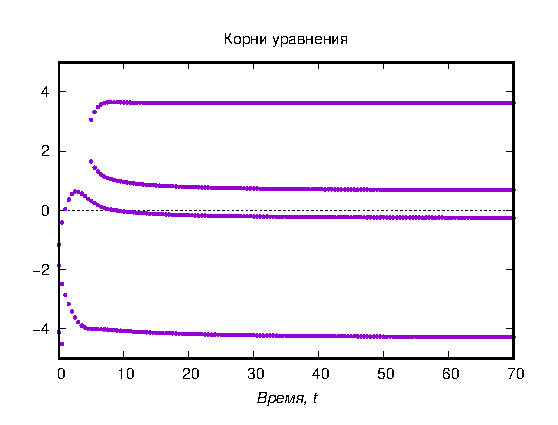
\includegraphics[width=0.7\linewidth]{roots1}}
	\caption{Корни при $\epsilon = 0.4$, $\omega = 0.8$}
	\label{ris:roots1}
\end{figure}

Из графика видно, что новых корней при большом отдалении ($t\gg0$) не возникает, а значит рассматривать отрезок такой длинны на появление новых корней не имеет смысла.

Чтобы убедится в этом построим график для других значений $\epsilon$ (рис. \ref{ris:roots2}):

\begin{figure}[h]
	\center{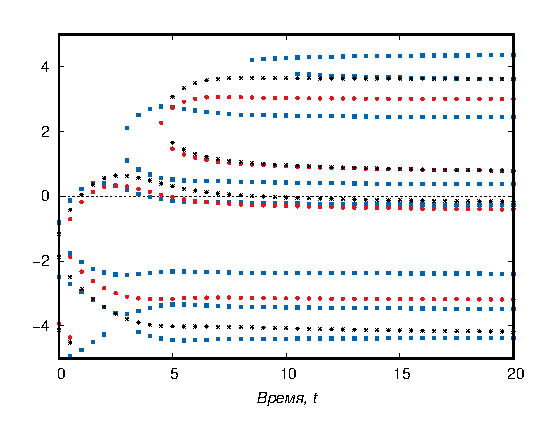
\includegraphics[width=1\linewidth]{roots2}}
	\caption{Корни при $\epsilon = $ 0.3 (квадраты), 0.35 (круги) и 0.4 (звездочки) }
	\label{ris:roots2}
\end{figure}

Видно, что для квадратов ($\epsilon = 0.3$) коней больше, чем для остальных параметров, максимум 6, и последний появляется при $t \approx 11$. Подобная закономерность просматривалась на графике (рис. \ref{ris:alpha-20..20}), где уменьшение $\epsilon$ привело бы к увеличению числа корней.

На рисунках (\ref{ris:full1}, \ref{ris:rootsend1} и \ref{ris:end1}) представлены графики сравнения решений для случая, когда $\epsilon = 0.4, F_0 = 2, \omega = 0.8$.

\begin{figure}[h]
	\begin{center}
		\begin{minipage}[h]{0.45\linewidth}
			\includegraphics[width=1\linewidth]{full1}
			\caption{Сравнение численного \textit{(обычная линия)} и аналитического \textit{(пунктирная)} решения. [0, 70]} %% подпись к рисунку
			\label{ris:full1} %% метка рисунка для ссылки на него
		\end{minipage}
		\hfill 
		\begin{minipage}[h]{0.45\linewidth}
			\includegraphics[width=1\linewidth]{rootsend1}
			\caption{Корни для аналитического решения }
			\label{ris:rootsend1}
		\end{minipage}
	\end{center}
\end{figure}

\begin{figure}[h]
	\center{\includegraphics[width=0.7\linewidth]{end1}}
	\caption{Сравнение численного \textit{(обычная линия)} и аналитического \textit{(пунктирная)} решения. [20, 70]}
	\label{ris:end1}
\end{figure}

Исходя из рисунка (\ref{ris:rootsend1}) можно сказать, что пики на графике аналитического решения (рис. \ref{ris:full1}) появляются в тех местах, где $t\approx t_0$ ($t_0$ - корень), в связи с тем, что множитель $\frac{1}{(t-t')^{3/2}}$ увеличивает значение функции на бесконечность.
Вблизи этих пиков мы не можем получить хорошую оценку, но если $|t-t_0|\gg 1$,  то аналитическая формула дает лучший результат, что видно на графике (рис. \ref{ris:end1}).

На рисунках (\ref{ris:full2}, \ref{ris:rootsend2} и \ref{ris:end2}) представлены графики сравнения решений для другого случая, когда $\epsilon = 0.4, F_0 = 2, \omega = 0.8$.

\begin{figure}[h]
	\begin{center}
		\begin{minipage}[h]{0.45\linewidth}
			\includegraphics[width=1\linewidth]{full1}
			\caption{Сравнение численного \textit{(обычная линия)} и аналитического \textit{(пунктирная)} решения} %% подпись к рисунку
			\label{ris:full2} %% метка рисунка для ссылки на него
		\end{minipage}
		\hfill 
		\begin{minipage}[h]{0.45\linewidth}
			\includegraphics[width=1\linewidth]{rootsend1}
			\caption{Корни для аналитического решения }
			\label{ris:rootsend2}
		\end{minipage}
	\end{center}
\end{figure}

\begin{figure}[h]
	\center{\includegraphics[width=0.7\linewidth]{end1}}
	\caption{Сравнение численного \textit{(обычная линия)} и аналитического \textit{(пунктирная)} решения}
	\label{ris:end2}
\end{figure}

Полученный аналитический результат так же достаточно хорошо описывает матричный элемент $\cM$, но как и говорилось до этого, точная оценка может быть получена не для всего временного промежутка времени. Сравнение графиков вблизи нуля показывает, что метод перевала не применим для случая $t\approx 0$, а также $t\approx t_0$. 
Стоит также отметить ожидаемый прирост производительности. Ускорение действительно велико, аналитическая оценка получается быстрее примерно в 10 раз. Эту цифру можно увеличить, если использовать более быстрые алгоритмы для поиска корней уравнения, чем метод Брента.

\sectionbreak
\section*{\centering{Заключение}}
\addcontentsline{toc}{section}{Заключение}

В ходе работы была получена асимптотические оценки для матричного элемента $\cM$, являющегося частью задачи моделирования атома под действием низко-частотного лазера, на основе метода перевала. 

Также работы было представлено описание метод перевала, и способ применения к задаче. Затем была получена асимптотическая оценка как сумма по всем перевальным точкам и показано, почему точка $t = 0$ вносит очень малый вклад в искомый интеграл. Разработана и реализована программный модуль на языке C++, использующий библиотеки FFTW и GNU GSL для получения численной оценки и сравнения ее с полученной аналитической формулой. Также описаны плюсы и минусы использования быстрого преобразования Фурье, в качестве инструмента интегрирования.

Анализируя результаты можно сделать вывод, что данная оценка позволяет качественно оценить данный интеграл, при условии $t \gg 0$, а также $t \gg t_0$.

Главной проблемой при оценке является ограниченность ее применения. Она не может получить хорошую оценку для случая, когда $t \approx 0$, а также $t \approx t_0$, где $t_0$ - корни уравнения $\alpha^2(t', t, t') = 2\epsilon$. Зато для случая, когда получение численного результата начинает занимать большое количество времени, и возникают проблемы точности, полученная формула работает хорошо. 

Можно было бы использовать для аналитических расчетов и аппроксимацию через функцию Эйри, для случая сливающихся корней, но в связи с тем, что корни близки только на том промежутке, на котором возникает сингулярность ($(t-t_0)^{-3/2}$), это не может принципиально улучшить оценку

Цель получить быструю качественную оценку была достигнута, ускорение составило порядка 10 раз. Причем можно сделать алгоритм еще быстрее, путем использования другого численного метода решения уравнения, так как почти все затраты ресурсов для получения оценки методом перевала занимает именно оно.


\newpage
\addcontentsline{toc}{section}{Список используемой литературы}
\bibliographystyle{utf8gost705u}  %% стилевой файл для оформления по ГОСТу
%\bibliographystyle{gost2008}
\bibliography{biblio}
% имя библиографической базы (bib-файла) 

\newpage
\addcontentsline{toc}{section}{Приложение А Листинг программы}
\section*{Приложение А\\Листинг программы}\label{attachA}

В данном приложении приведена текст программы, реализующий алгоритмов, приведенных в данной работе.

\lstinputlisting[language=C]{main.c}

\end{document} 